\documentclass{beamer}
\hypersetup{unicode}
\usepackage[utf8]{inputenc}
\usepackage[croatian]{babel}
\usepackage{csquotes}
\MakeOuterQuote{"}
\usepackage{thmtools}

\usepackage{datetime}
\newdate{date}{08}{06}{2024}
\date{\displaydate{date}}

\declaretheorem{teorem}
\declaretheorem[style=remark, sibling=teorem]{primjer}
\declaretheorem[style=remark, sibling=teorem]{napomena}
\declaretheorem[style=definition, sibling=teorem]{definicija}

\usepackage[style=authoryear]{biblatex}
\addbibresource{literatura.bib}
\usepackage{tikz}

\usepackage{listings}


% manage colors: https://www.r-bloggers.com/2011/11/create-your-own-beamer-template/
% and https://ramblingacademic.com/2015/12/08/how-to-quickly-overhaul-beamer-colors/

\usetikzlibrary{arrows}
\newcommand{\midarrow}{\tikz \draw[-triangle 90] (0,0) -- +(.1,0);}

\definecolor{seagreen}{HTML}{21b2aa}
\definecolor{magenta}{HTML}{b2217f}
\definecolor{gold}{HTML}{ca9520}
\definecolor{red}{HTML}{da272f}
\definecolor{blue}{HTML}{4682b4}
\definecolor{purple}{HTML}{a65cef}

\definecolor{white}{HTML}{ffffff}
\definecolor{dwhite}{HTML}{eeeeee}
\definecolor{black}{HTML}{000000}
\definecolor{lblack}{HTML}{222222}

\colorlet{bgmain}{seagreen}
\colorlet{bgsec}{magenta}
\colorlet{bgter}{gold}
\colorlet{fgmain}{black}
\colorlet{fgsec}{lblack}

\usetheme{Madrid}
\usecolortheme{orchid}
% \useinnertheme{rounded}

\setbeamercolor{titlelike}{parent=structure, bg=seagreen, fg=white}
\setbeamercolor{palette primary}{bg=magenta, fg=white}
\setbeamercolor{palette secondary}{bg=magenta, fg=white}
\setbeamercolor{palette tertiary}{bg=magenta, fg=white}
\setbeamercolor{palette quaternary}{bg=magenta, fg=white}
\setbeamercolor{structure}{bg=white, fg=magenta} % itemize, enumerate, etc
\setbeamercolor{section in toc}{fg=black, bg=lblack} % TOC sections
\setbeamercolor{frametitle}{fg=white, bg=seagreen}

\setbeamercolor{block title}{fg=white, bg=seagreen}
% \setbeamercolor{block body}{bg=white, fg=white}

% Override palette coloring with secondary
\setbeamercolor{subsection in head/foot}{bg=seagreen,fg=white}

\lstdefinestyle{mystyle}{
	backgroundcolor=\color{white},
	commentstyle=\color{magenta},
	keywordstyle=\color{seagreen},
	stringstyle=\color{magenta},
	basicstyle=\ttfamily\footnotesize,
	breakatwhitespace=false,
	breaklines=true,
	captionpos=b,
	keepspaces=true,
	numbers=none,
	showspaces=false,
	showstringspaces=false,
	showtabs=false,
	tabsize=2
}
\lstset{style=mystyle}

\title[PyGDB]{PyGDB --- analiza strukture izvornog koda}
\subtitle{Projekt iz kolegija Napredne baze podataka}
\author{Luka Šimek}
\institute[PMF--MO]{Prirodoslovno-matematički fakultet --- Matematički odsjek\\Sveučilište u Zagrebu}
\date{\displaydate{date}}

\begin{document}
% \nocite{*}

\begin{frame}[plain]
\titlepage
\end{frame}

\begin{frame}{Sadržaj}
\tableofcontents
\end{frame}

\section{Motivacija}
\begin{frame}{Motivacija}
\begin{itemize}
\item vrhovi: paket, modul, klasa, funkcija, ime
\item odnosi: uvoz, nasljeđivanje, nazivni prostori, pridruživanja, atribut, metoda, tip...
\item putevi: hijerarhije datoteka, klasa, opsega, uvoza
\item upiti: filtriranje nepregledne količine podataka
\item \( \Rightarrow \) grafovska baza podataka
\end{itemize}
\end{frame}

\begin{frame}{Primjer}
\begin{figure}
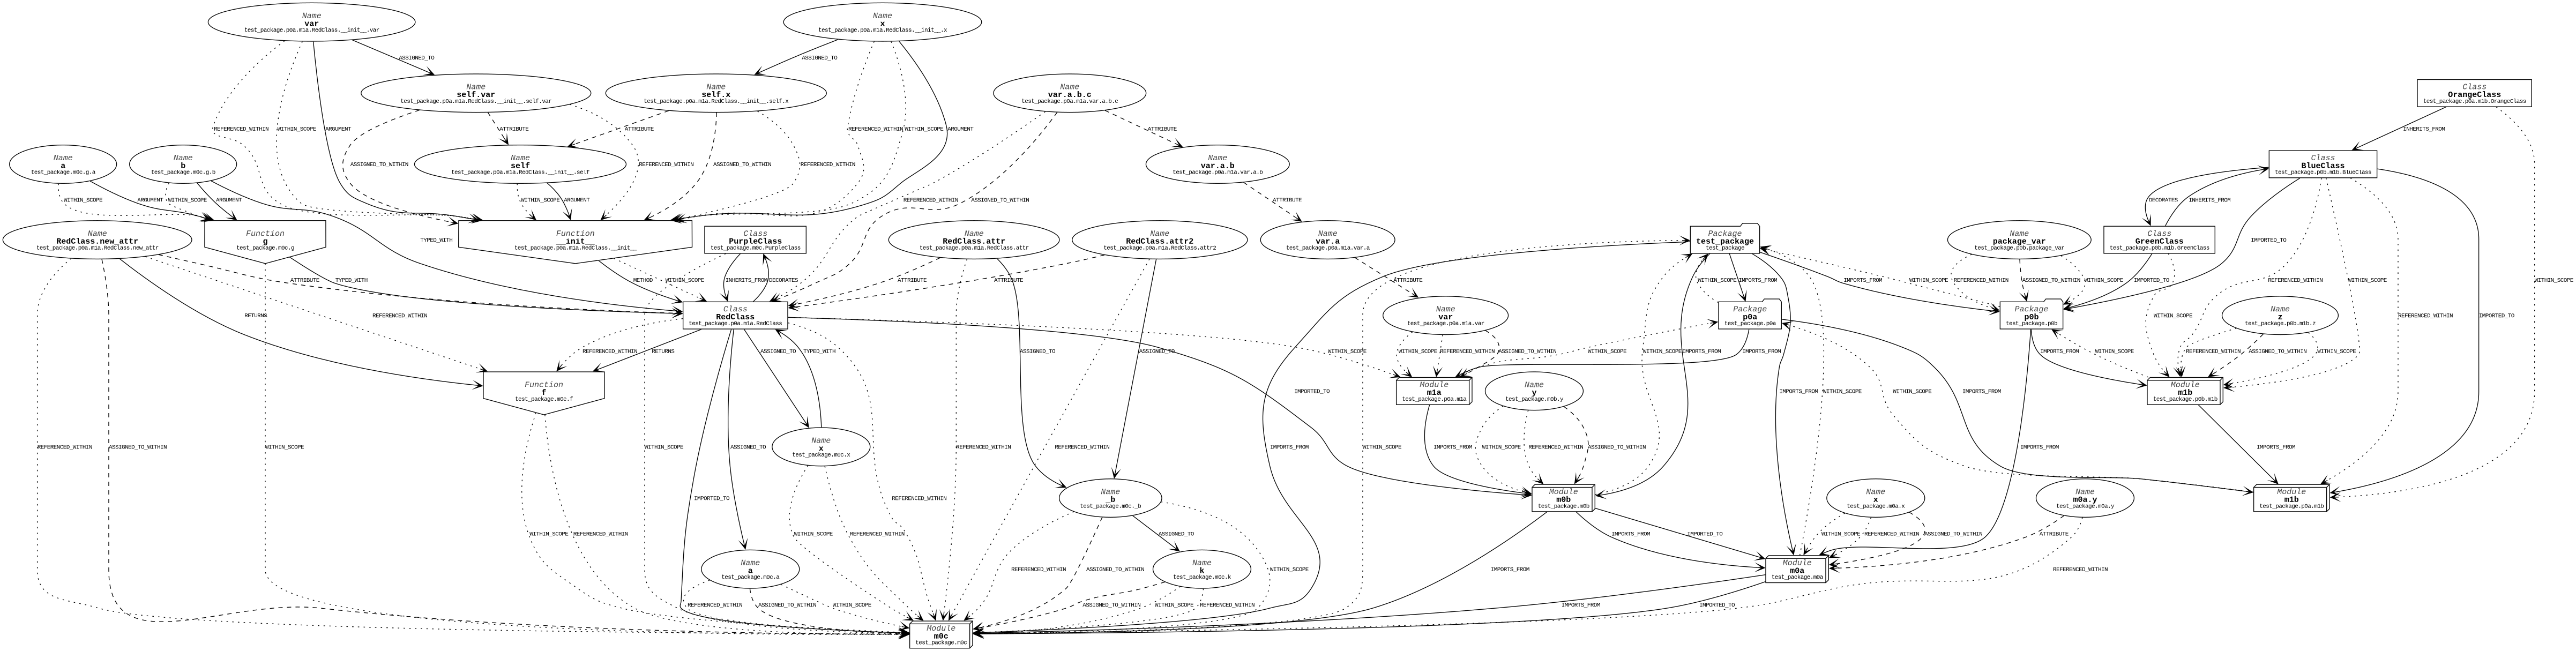
\includegraphics[scale=0.1]{assets/testni.png}
\centering
\caption{Graf testnog paketa (60-tak linija ukupno)}
\label{fig:primjer}
\end{figure}
\end{frame}

\section{Pokazna baza}
\begin{frame}{Pokazna baza}
Unosimo u bazu grafove 5 paketa:
\begin{columns}
\column{.5\textwidth}
\begin{itemize}
\item ovaj projekt,
\item humanize,
\item Requests,
\item Seaborn,
\item PyMC
\end{itemize}
\column{.5\textwidth}
...oko 30K vrhova i 220K bridova
\end{columns}
\end{frame}

\begin{frame}[fragile]{Primjeri upita}

\begin{itemize}
\item sve rekurzivne funkcije
\begin{lstlisting}
MATCH (f: Function)-[b:RETURNS]->(f)
RETURN f, b;
\end{lstlisting}

\item nasljeđivanje u paketu Requests
\begin{lstlisting}
MATCH (p: Package {fullname: 'requests'})
MATCH (p)<-[:WITHIN_SCOPE*]-(c: Class)
MATCH (c)-[b:INHERITS_FROM*1..]->(d: Class)
RETURN c, b, d;
\end{lstlisting}

\item klase unutar ovog projekta i kad se \enquote{spominju}
\begin{lstlisting}
MATCH (p: Package {fullname: 'pygdb'})
MATCH (p)<-[:WITHIN_SCOPE*]-(c: Class)
MATCH (c)-[b:REFERENCED_WITHIN]->(d: Class)
RETURN c, b, d;
\end{lstlisting}

\end{itemize}
\end{frame}

\begin{frame}{Primjer rezultata}
\begin{figure}
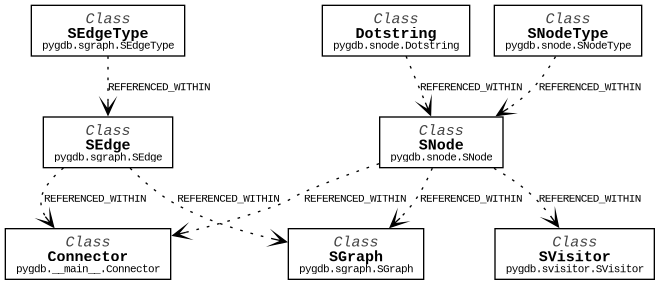
\includegraphics[scale=0.5]{assets/klref.png}
\centering
\caption{Rezultat trećeg upita}
\label{fig:2}
\end{figure}
\end{frame}

\section{Osvrt}
\begin{frame}[fragile]{Nedostaci}
Statička analiza u dinamičkom jeziku:
\begin{itemize}

\item dinamički tipovi
\item dinamički generirani kod (\texttt{exec}, \text{setattr}, modul \texttt{importlib}...)
\item FFI
\end{itemize}

\end{frame}

\begin{frame}[t]{Literatura}
\printbibliography
\end{frame}
\end{document}

